\documentclass[12pt,halfline,a4paper,nonumbib]{ouparticle}

%\usepackage[authoryear]{natbib}

\usepackage[backend=biber,
            style=authoryear,
            %citestyle=authoryear,
            maxcitenames=1,
            sorting=nyt]{biblatex}
\addbibresource{references.bib}

%% My definitions
\usepackage{xcolor}
\newcommand{\todo}{\textcolor{red}}
\newcommand{\disp}{\displaystyle}

\usepackage{algorithm}
\usepackage{algorithmicx}
\usepackage{algpseudocode}

\usepackage{setspace}
\doublespacing

\usepackage{lineno}
\linenumbers

\usepackage{subcaption}


\begin{document}


\iffalse
\section{Resubmission Proceedure}

To revise your manuscript, log into https://mc.manuscriptcentral.com/icesjms and enter your Author Centre, where you will find your manuscript title listed under "Manuscripts with Decisions."  Under "Actions," click on "Create a Revision."  Your manuscript number has been appended to denote a revision.

You will be unable to make your revisions on the originally submitted version of the manuscript.  Instead, revise your manuscript using a word processing program and save it on your computer.  Please also highlight the changes to your manuscript within the document by using the track changes mode in MS Word or by using bold or colored text.

Once the revised manuscript is prepared, you can upload it and submit it through your Author Centre.

When submitting your revised manuscript, you will be able to respond to the comments made by the reviewer(s) in the space provided.  You can use this space to document any changes you make to the original manuscript.  In order to expedite the processing of the revised manuscript, please be as specific as possible in your response to the reviewer(s).

IMPORTANT]  Your original files are available to you when you upload your revised manuscript.  Please delete any redundant files before completing the submission.

Please ensure that the manuscript conforms to the ICES JMS formatting requirements, particularly the resolution and sizing of the Figures (which should be designed to fit the page format of the Journal).

Because we are trying to facilitate timely publication of manuscripts submitted to the ICES Journal of Marine Science, your revised manuscript should be uploaded as soon as possible.  If it is not possible for you to submit your revision in a reasonable amount of time, you may request a short extension of time by emailing the  editorial office.

Once again, thank you for submitting your manuscript to the ICES Journal of Marine Science and I look 



\section*{Review}

\subsection*{Editor's Letter}

Manuscript ID ICESJMS-2020-419 entitled "Validation of stock assessment models. Is it me or my model talking?" which you submitted to the ICES Journal of Marine Science, has been reviewed.  The comments of the reviewers are included at the bottom of this letter. 

The reviewers have recommended publication only after major revisions to your manuscript. Most of the comments are minor but reviewer 1 said that he did not “think the work included in the manuscript is sufficient to support all the conclusions”. Also reviewer 2 has some major comments. My own, minor, comment is that the writing is not always clear and some sentences are not even grammatical. Our editor in chief reminded me that we discourage article titles to contain questions rather than declarative statements. Moreover, the question in the title is not even very clear. 

Therefore, I invite you to respond to the reviewers' comments and revise your manuscript. Please submit your revision by 23-Nov-2020.

\subsection*{Response}

Dear Sarah

Thank you for the review. We were pleased the reviewers found the paper thought provoking. However, they also identified the need for clarification and made suggestions for additional work. We have gone through your recommendations and their comments carefully and restructured the manuscript as suggested, clarified sources of misunderstanding, and deleted sections that were thought to be superfluous. We note that there was no consensus among the reviewers for some of the comments, other than the value of the work. We felt that some of the comments were because we are introducing methods that, although widely used in fields such as energy and climate modelling, are currently not routinely used in fisheries stock assessment.  Where we have not accepted the reviewers recommendations we have provide justification for not doing so. 

Our approach was based on validation and prediction skill. Where prediction skill is a measure of the accuracy of a forecasted value compared to the actual (i.e. observed) value that is not known by the model. There appeared to be some confusion about what was meant by prediction, since the reviewers appeared to have thought that, like in a stock assessment working group this was a two stage process, i.e. first fit to the data then project for management measures. We did not do this, our procedure was similar to a jackknife where we removed points using a tail cut or peel then "predicted" missing values. This means that we did not have to make assumptions about recruitment and catch, and could estimate prediction skill for any data series and observation. Also validation is not a binary process, i.e. valid/invalid, as there is a continuum between the two extremes which requires an iterative process  to examine if a model family should be modified or extended. We were not trying to identify a "best assessment" therefore, but to identify if models were overfitted,  whether it is plausible that the data were generated by a system identical to the model, and if not how they could be extended to better describe the dynamics. We were also not proposing validation as the only diagnostic tool to be used in stock assessment, but as a key tool for use in the stock assessment toolbox. We hopefully have now clarified all these points in our response.

With respect to the missing reference, \cite{brooks2016retrospective} used model based quantities not observations. It was therefore a test of consistency within a model, not validation as they did not use observations to estimate prediction skill, they also conducted a two stage process where additional assumptions had to be made about the future, and relative error. These are important differences which we now explain more clearly in the manuscript.

Regarding the comments about catch advice, this appears to be another misunderstanding, since as part of the hindcast approach the reported catches are used to compute missing observations. We do accept that the impact on catch advice is important, but we argue that this is best conducted using Management Strategy Evaluation. We therefore have another follow up paper that combines the hindcasting approach with MSE \parencite[e.g.][]{pastoors2007validating}.

The reviewer's comment about not supporting "all the conclusions", is perhaps due to a misunderstanding. The reviewers appears to want us to identify a "best assessment". Validation, however, is not a binary process and should be used alongside other methods. Furthermore, we did not want to undermine the work of the IOTC scientific committee, as we recognise that the stock assessment process has to take many factors into account, when agreeing an assessment. Validation is an important, but not the only, tool in this regard particularly as it increases trust in that it is the model talking. We have another paper in review which demonstrates the use of validation as part of the process of identifying a "best assessment" \cite{carvalho2020cookbook}. That paper is provided as a reference and if desired we can send a copy of the paper to support our argument. 

One reviewer states the importance of alternative SS parameterisations and scenarios, while another questions the use of ensembles of multiple models. Using an ensemble (or grid) of models is a common way in the tuna world when providing catch advice and conditioning Operating Models as part of Management Strategy Evaluation. It is also widely used in fields like climate modelling. The reviewer who suggested deleting the reference to ensemble models actually suggests a way of weighting models based on prediction skill. So it appears that it is recognised it is an important research area where model validation can be used. This is something that for example ICES has started to address (see 2021 ASC theme  session M and WKENSEMBLE and WKGMSE3 workshops). This is why we included the discussion of ensemble models and suggest prediction skill as a way of weighting or rejecting models. Again this is a topic that we are currently working on for a follow up paper, and so we think the reference to ensemble models is justified.

We agree with the comments about the need for a simulation exercise, and we are currently designing a study that will address the issues identified by the review. This, however, is beyond the scope of the current paper. This study is a proof of concept and provides a description of how we can evaluate alternative models using prediction skill.

With respect to the subtitle "me or my model talking" this was a homage to the Hodge and Dewar paper, "Is it you or your model talking", but we were afraid of sounding arrogant so changed from the second to the first person. It and our definition of stock assessment were also intended to promote debate. A reviewer stated they liked the subtitle and so we would like to keep it, as it helps support our definition of prediction skill, but have changed the main title to "Validation of stock assessment models using prediction skill" to make the link clearer.
\newpage

\seection{Response to Reviewers}

\subsection*{Reviewer 1}

\subsubsection*{General Comments}

\begin{itemize}
    \item I found this manuscript to be thought provoking and believe that it addresses a worthwhile topic. I also strongly agree with the underlying premise and motivation for this manuscript, namely that the predictive capabilities of assessment models should be given increasing consideration relative to goodness of fit diagnostics. 
    \textit{\newline We agree with this. Thank you!}

        \item I would have liked to have seen a follow up SS run with the length composition removed or down weighted and a demonstration that the validity improves. 
    \textit{\newline We ran an SS scenario where we down weighted the length data (effective sample size was 0.00005) and the results were very similar to the ASPM. However, we don't show this in the paper as we are not developing a best model.}

    \item The ultimate goal of projections in stock assessment is also catch advice. I would suggest a demonstration that a model that is generally valid produces more accurate catch advice. This could be achieved with an expansion of the existing methods to include catch advice in the hindcasting period or through a broader and more general simulation study.
    
    \textit{\newline We could not use the approach of \cite{brooks2016retrospective} as the estimates of model based quantities such as "SSB" can not be used for validation. In a follow on paper we conduct an MSE using a backtesting procedure to address this issue.}

    \item My main concern, however, is that I do not think the manuscript did enough to sufficiently demonstrate the utility or usefulness of the proposed hindcast method. I also do not think the work included in the manuscript is sufficient to support all the conclusions. For example, the SS model was generally found to be “invalid”, which the manuscript attributes to length composition data. But, I can theorize several other reasons for why the SS model might be invalid (e.g., recruitment penalty in the likelihood, overparameterization given that the model is likely estimating thousands of parameters).
    \textit{\newline The intention was not to come up with a "best assessment" but a method that can be used to help validate candidate hypotheses and show where the model should be extended. 
    Validation is not a binary process, i.e. valid/invalid, as there is a continuum between the two extremes which requires an iterative process. We were therefore not trying to identify a "best assessment", but to identify if models were overfitted,  whether it is plausible that the data were generated by a system identical to the model, and if not how they could be extended to better describe the dynamics. We were not proposing validation as the only diagnostic tool.  We are addressing the issues raised by the reviewers comments in other papers e.g. \cite{carvalho2020cookbook}. The ambition of validation is not to prove that a model is correct, but to check that the model cannot be falsified with the available data. This requires extending the model to include relevant hypotheses, collection of appropriate data, and improved knowledge.   For example a trend in a recruit index of abundance could be explained by an increase in recruitment or a reduction in natural mortality, while a trend in an adult index by senescence or a change in selection pattern. We believe that the approach we demonstrate can help. We also did not want to usurp the role of the IOTC scientific committee who have to consider the bigger picture when they agree on an assessment.}

    \item Lastly, I think the manuscript could be much improved by restructuring much of the text, especially between the introduction and methods sections. I expand on these and other topics in the more specific comments below.
    \textit{\newline We have now restructured the model.}

\end{description}

\subsubsection*{Specific Comments}

\begin{description}
\item[Brooks and Legault, 2016] used a similar hindcasting method as that used in this study. I suggest citing that work. Brooks, E.N., and Legault, C.M. 2016. Retrospective forecasting] evaluating performance of stock projections for New England groundfish stocks. CJFAS 73] 935-950. dx.doi.org/10.1139/cjfas2015-0163. 
\textit{\newline Now cited, but Brookes and Legault (2016)  used model based quantities and evaluated stability within a model.  A model can only be validated if it is able to predict observations not used when fitting the model.  As demonstrated here this needs to be based on observations, i.e. is a model free exercise, and creates a platform for evaluation across alternative model structures.}

\item[Line 74-75] Expand on why this can be challenging.
\textit{\newline See next comment.}
\item[Line 120-142] All this could likely be moved to the introduction, and portions of it could be used to resolve the expansion I suggest for lines 74-75.
\textit{\newline Moved to introduction and addresses challenges.}

\item[Line 143-146] I suggest describing the assessment models first, then describe the hindcasting procedure. I think this change would make the methods more consistent with the chronology of the research.
\textit{\newline This has now been done.}

\item[Line 147] It is not clear from this sentence exactly what the main objective is, and so I suggest stating it more explicitly.
\textit{\newline The objective is now clearly stated as "The objective of the paper is validation of models using prediction skill, defined as a measure of the accuracy of a forecast value compared to an  observed value that is not known by the model (i.e. model-free validation). Current literature primarily focuses on the past, and how well models fit these data. Historical performance, however, is no indicator of how well a model may perform in the future."}

\item[Line 156-205] This section switches between describing a base case SS model and providing other background on the fishery and stock status. I suggest moving everything associated with background and stock status to the end of the introduction or give all of this contextual information its own section at the top of the methods. I also assumed that this was a description of the SS model used for the research, but that is never explicitly stated. This lengthy SS description also seemed bizarre here because there is a separate subsection just for Assessment Methods.
\textit{\newline Text has now been restructured, so that 1st assessment methods are described, then the data used for the assessment are summarised as suggested above.}

\item[Line 172-181] When discussing the spatial regions, I suggest using the “R-number” as they appear in Figure 1.
\textit{\newline Done}

\item[Line 190-192] Expand on why the length composition data is used in this way. The length comp data being used this in the SS fit also seems contradictory to the conclusion that this data is causing the SS model to be generally invalid. If length comp is not affecting trends in stock abundance then how is it the source of the validity problems? As in my general comments, I suggest exploring this further.
\textit{\newlineThis is a valid point, since validation can be performed using any data not used in fitting and this includes length composition data. We did attempt validation using length composition data, however, as an aim of the study was to demonstrate how to compare models from different families, and the biomass dynamic model does not use length data. This will be the subject of a further study, i.e. to evaluate integrated models with different structures and data weightings.}

\item[Line 196] need a period after fleets.
\textit{\newline Added}

\item[Line 200] need a period after time.
\textit{\newline Added}

\item[Line 210-216] This can likely be deleted.
\textit{\newline Deleted}

\item[Line 217] I was not sure what this description is an example of.
\textit{\newline It is no longer described as an example but is a description of the ASPM.}

\item[Line 231-235] This paragraph is two sentences that are seemingly unrelated. I suggest revising or deleting.
\textit{\newline Deleted.}

\item[Line 246] The phrase tuned to the base case SS assessment suggests the JABBA model was fit to the biomass estimates from SS. If true, then why? I would have thought JABBA would be fit to the raw catch and index data. Please expand on this topic here.
\textit{\newline This has now been clarified as "priors for the production function parameters were on the SS base case"}

\item[Line 276] The algorithm did not help me at all to understand the methods. It can likely be deleted.
\textit{\newline Deleted}

\item[Line 295] I would suggest using a symbol other than xxx here to more easily distinguish these projected
values from the estimated values of the retrospective analysis in the previous section.
\textit{\newline We have made the definition of MASE more generic, and so have deleted the 2nd equation..}

\item[Line 296] change (1,t) to (1:t).
\textit{\newline Done}

\item[Line 314] MAPE is never defined. I suggest deleting this comparison to MAPE.
\textit{\newline Deleted}

\item[Line 321 and Figure 3] The labels in Figure 3 are “stock” and “harvest”, which here I think are SSB and F. I suggest changing the Figure to be consistent. In the top two rows of Figure 3, the thick black line is described as the estimates from the full time series, but there is a light blue line that extends beyond the thick black line in some of the panels. Shouldn’t the thick black line be the longest time series? I think something is wrong or perhaps I’m misunderstanding. I generally found Figure 3 cumbersome and
difficult to understand, but I do not have any great suggestions for a solution.
\textit{\newline We can not change the legends by row, that is why we used stock and harvest to make them more generic. We have now defined the quantities in the legend. We agree that the figures show a lot of information, and have simplified these now.}

\item[Line 329-331] I wondered here whether any ASPM model would ever have a significant retrospective pattern. So much of the model is fixed and deterministic that it’s hard to imagine a systematic change in the time series estimates as less data are used. I suspect the ASPM would sacrifice fit to the indices as it has no ability to estimate a different biomass trend. This degradation in fit is of course the whole point, but it makes examining the retrospective pattern a bit moot. If my logic here sounds reasonable then perhaps just add a caveat to the discussion.
\textit{\newline This is an important point and is why we used prediction skill based on observations. For example if SS was used as a catch only method \parencite[e.g. Simple SS][]{cope2013implementing} and a retrospective analysis run, then if parameters were fixed or had highly informative priors then there may be no retrospective pattern, even if the model was totally wrong. For example if a catch only method with herring priors was used with data from cod. This is why validation should be done using observations not included in the model. We make this point in the manuscript.}

\item[Line 332] I am not clear on why these methods are considered “model-free”. Everything seems dependent on a model to me. Perhaps either explain further or change the terminology. 
\textit{\newline To clarify we now Define Prediction Skill as "Any measure of the accuracy of a forecasted value compared to the actual (i.e. observed) value that is not known by the model" state that you can only validate models on observations, Then rather than saying model free or model based we refer to "prediction skill"}

\item[Line 335] I think prediction skill was poor for indices 2 and 4, not 2 and 3. Correct?
\textit{\newline Yes, now corrected}

\item[Line 338] This sentence is the only place where the term horizons is used in this context, which made it confusing. Perhaps re-word.
\textit{\newline horizon is now defined before it is used.}

\item[Line 342] The use of length comp is not the only difference between SS and ASPM and so I’m not clear on the logic or intention of this sentence.
\textit{\newline This has now been clarified, i.e. "ASPM is parameterised based on the selectivity estimated by a "full" SS model. The model is then fitted to the abundance indices, assuming a deterministic spawning recruitment relationship, and without the size composition data contributing to the likelihood function."}

\item[Line 343-344] The logic supporting this last sentence is not clear. The preceding sentences just note a few difference between the three models, but no analysis or results are referenced in support of the conclusions in the last sentence. This logic needs to be made much clearer. Also, I wondered here if an implication of the results is that you can have a “valid” model with good prediction skill that is premised on an invalid model. ASPM had the best prediction skill but it uses estimates from the SS model. Does the poor prediction skill of SS also invalidate ASPM given that it depends on SS?
\textit{\newline We have made it clear that the objective of validation is to check that the model can not be falsified with the available data, and validity is a continuum. Therefore we are really saying  how useful a model is in prediction. With respect to ASPM being dependent on SS, we could have looked at alternative ASPM parameterisations, e.g. dome shaped verses flat-topped selection patterns, or different levels of natural mortality. We did not do this as we wanted three "relatively" simple examples that presented a continuum to help demonstrate the concept. We were also not attempting to find a best assessment.}

\item[Line 375] Add a corresponding region number that references Figure 3 for the Eastern Indian Ocean Region.
\textit{\newline Done}

\item[Line 407] I like the “is it me or my model talking” catch phrase, but I think the point is that the somewhat subjective decisions we make in stock assessments might create an invalid model and we need to be checking for these things via prediction skill. That point is not clear here, which makes the catch phrase less impactful. I suggest just expanding on the meaning of the catch phrase.
\textit{\newline We have have now clarified this in the conclusions, i.e. 
As the stock assessment process become more complex, e.g. through the increased use of integrated models, ensembles of models, and Management Strategy Evaluation, there are concerns about a lack of transparency. This is because of the many internal, implicit and often poorly documented assumptions, and a lack of access as only a few highly skilled experts are able to run the models \citep{hilborn2003state}. Therefore to increase confidence in the outputs of a model and trust amongst the public, stake and asset-holders and policymakers it is important for modelers to ask “is it me or my model talking” before others ask the question posed by \cite{hodges1992you} "you or your model talking?".} 

\item[Line 459] The general benefits to doing this type of hindcasting are not sufficiently described anywhere in the manuscript. Is the point to ID lousy data (like in this manuscript), eliminate families of models from consideration, something else? I think the introduction touches on this a little, but it is not clear.
\textit{\newline We have now clarified that the objective is not to prove that a model is correct, but to check that the model can not be falsified with the available data. In other words if a model has poor prediction skill then you either need more informative data or to develop alternative models. This is a step forward from hypothesis testing and model selection which is a way of rejecting rather than extending models. We have made this clearer in the introduction.}

\item[Line 461] I thoroughly enjoyed the fact that this research was put in the context of a conversation with Sidney.
\textit{\newline Thanks}

\item[Figure 2] is never referenced in the body of the manuscript and can be deleted. The column titles “method” and quantity need to be reversed in Table 1.
\textit{\newline Figure 2 has been deleted. Table corrected.}

\end{description}

\newpage
\subsection*{Reviewer 2}OK

\subsubsection*{General}

\begin{itemize}
    \item This paper advocate for the so-called hindcast measures as an alternative to the retrospective measures which are routinely used to validate fish stock assessment models. This is a good idea in its own right. The measures are clearly defined and well reasoned. The authors are rightfully sceptical w.r.t. prediction of model outputs (such as biomasses and fishing mortality measures). The emphasis should be on predicting observed quantities.
    \textit{\newline Thanks for the endorsement.}

    \item Not all assessment models are really capable of predicting into the future based purely on the model used for the assessment - if for instance, the model requires new yearly parameters, then the model itself cannot predict. In that case, forward projections require additional assumptions and in that case, it is debatable if we are validating the model or the additional forecast assumption. This detail deserves to be mentioned.
    \textit{\newline We did not perform projections as a two part process as implied by the reviewer. We omitted observations from the recent period, fitted the model and predicted the missing values.  This is similar to a jackknifecool, th edifference was that we peeled back from the terminal year when deleting observations. A problem with the jackknife, however,  is serial correlation. That is why we  performed a hindcast. %If you can not predict observations how can you validate a model? For example Catch-only-methods that only use catch, if you remove catch then you can not fit that year, so is the method invalid?
    }

    \item In e.g. an age-based assessment there will typically be the different observation uncertainty for different age classes, hence it should be expected that certain age classes will be easier to predict. The current approach uses a raw average of all prediction errors, but that could (and likely will) make the proposed measure dominated by a single age class (e.g. the smallest), which seems unfair. A better measure would penalize small deviations from precise observations more and penalize large deviations from imprecise measurements less.
    \textit{\newline You can use prediction skill for any quantity that is observable and can be predicted by a model. This could be an age class if those data are available. MASE has the desirable properties of scale in-variance so can be used to compare forecasts across data sets with different scales.}

    \item This one I may have misunderstood, but it seems to be implied that contrary to AIC hind-casting can also be used to compare models working on different data series. I don't see for it can be used to compare e.g. a model fitting to a biomass series to a model fitting to an age?
    \textit{\newline AIC can only be used to compare models based on the same input data, this is now stated clearly. }

    \item The idea of using these prediction measures as weights in an ensemble model (or weights in operating models) is mentioned several times but not followed through. That idea does not appear feasible, the paper does not document that it is, and does not provide any details. I would suggest dropping that part of the manuscript.
    \textit{\newline simple prediction skill is widely used elsewhere, we have provided references \parencite[i.e.][]{ianelli2016multi, casanova2009weighting}}. We address this in a follow on paper, so have left the reference to ensemble modelling.}

    \item The basic problem is that these models overlap. So we can imagine two models predict equally well and hence should be given equal weight half-half. Then imagine 10 models] First model is the first of the two models above and the remaining nine models are slight variations of the second model above. Now all 10 predict equally well and hence should each get 1/10 of the weight, but effectively we will end up with giving 90\% weight to the second model and 10\% weight to the first.
   \textit{\newline A main issue is the initial choice of models, we address this in our next paper.}

    \item To solve this problem we should be able to estimate covariances in the prediction errors (to get a first approximation of the overlap), and then weight accordingly to that, but is fisheries time series we are very unlikely to get time-series long enough to estimate such covariance matrices.   
    \textit{\newline The reviewer proposes a way of weighting that could be investigated using the approach in the paper. We used twenty years for the hindcast period, and could calculate the covariance. However, covariances are affected by the scale, so it may be better to use correlations. This is a potential research area, and so we would like to keep the reference to ensemble models in the paper.}
    
    %A key point is that validation is not binary i.e. pass/fail, as there is a continuum between these two extremes. So the objective is not to come up with a best assessment, and several models may pass the check that the model cannot be falsified with the available data. In which case advice needs to take this into account, i.e. Kobe PP \cite{kell2016quantification}.
    
    
    %There are many potential error metrics, and the best statistical measure to use depends on the objectives of the analysis and using more than one measure can be helpful in providing insight into the nature of observation and process error structures \parencite{kell2016xval}.
    
    %For example a commonly used measure is root mean square error. As the square root of a variance it can also be interpreted as the standard deviation of the unexplained variance, lower values indicate better fits. $E^\prime$ is sensitive to outliers, however,and favours forecasts that avoid large deviations from the mean and cannot be used to compare across series.  For example the correlation ($\rho$) between $Y_y$ and $\bar{Y_y}$ is not affected by the amplitude of the variations, is insensitive to biases and errors in variance, and can be used to compare across series. $E^{\prime 2}$ and $\rho$ are related by the cosine, and so could be summarised in a single diagramme, for simplicity, however, we settled on MASE.
    
    %MASE was chosen because it has the desirable properties of scale invariance, predictable behaviour, symmetry, interpretability and asymptotic normality. MASE does not skew its distribution even when the observed values are close to zero. MASE is also easier to interpret as a score of 0.5 indicates that the model forecasts are twice as accurate as a na\''{i}ve baseline prediction; the model thus has prediction skill.

    \item The prediction measure does not take into account how similar or different the models are, and assessment are often very similar (slight variations of the same basic model).
    \textit{\newline The reviewer is correct it does not, and we say nothing about model complexity. However, we do implicitly address overfitting, a problem with models with many parameters.}

    \item (in the text somehow all less than symbol "<" was turned into "!" in my version?)
    \textit{\newline done}

\end{itemize}


\subsubsection*{Specific Comments}

\newpage
\subsection*{Reviewer 3}
\subsubsection*{General}

\begin{description}
    \item Stock assessment models have increased in complexity and may use a wide array of data that needs to be properly weighted in the objective functions used to estimate the parameters, to avoid the risk of biasing the results. Thus, new diagnostic tools are a welcome addition to the toolbox of stock assessment modelers, to help detect model misspecification and appropriate weighting of different data set. The hindcast diagnostic proposed by the author seems interesting as model diagnostic and as a way of ranking models.  I find the manuscript interesting because there is a need for diagnostics for stock assessment models and it is a field that is very active, with several different diagnostics been proposed in recent years. The authors demonstrated that the hindcasting diagnostic detected differences in the prediction ability of different stock assessment models that were not detected by retrospective analyses. The authors conclude that the ASPM is a better model to assess the yellowfin tuna in the Indian Ocean judging by the hindcasting diagnostics. All models had similar retrospective patterns; thus, the hindcasting seems to be superior for differentiating among models. I believe the manuscript would be of interest to the reader of ICES JMS. I recommend the publication of the paper after the authors perform some revisions to improve clarity.
    \textit{\newline Thanks}

    \item The definition of stock assessment put forward by the authors (“The description of the characteristics of a 'stock' so that its biological reaction to being exploited can be rationally predicted and the predictions tested, Holt) seems to be a good operational definition that allows for practical developments such as the proposed of diagnostics. However, I feel that not all stock assessments have the goal of predicting, some have the main goal of estimating the status of the stock in relation to pre-defined reference points while acknowledging that prediction may be an unattainable goal. In the case of the goal not being that of predicting, what would be the advantage of the proposed hindcast diagnostic?
    \textit{\newline In the hindcast we looked at one step and three step ahead predictions by conducting a peel. We did no go beyond the range of the data, so we actually addressed the reviewers concern. We have now made this clear.}

    \item The main goal of the paper and the connection to the title should be stated more clearly at the end of the introduction. In Line 115, the authors state] “as a working example, we compare three model families etc…” what is the connection between the title and the goals of the paper? “When is “me” talking versus the model talking? When the model cannot be used to predict? So if the models do not pass the validation, it is “me” talking? Some of the text at the end of the abstract plus some text from the methods section (Line 147 to 149) can be used to word the main goals of the manuscript by the end of the introduction section.
    \textit{\newline We have added a sentence in the end of the Introduction that covers this comment

    \item It is not completely clear how the hindcasting is computed, in the explanation in the text the authors talk about predictions but in Line 276 where the algorithm is stated, there is no step related to predictions. How are the predictions obtained for each of the three stock assessment models? Are the actual catches by fishery and area for the year that been predicted used? Or the fishing mortality is held at the values from the previous year or average for a group of years? Also, what recruitment deviations by area and time are used for the predicted years? Are those set to zero? Or it is a sample from the previous years? Those details need to be explained more clearly, to be able to assess whether the hindcasting is diagnosing the actual assessment model rather than the projection algorithm.
    \textit{\newline There was no actual "projection", observations were removed by tail cutting and then missing values predicted.}

\end{description}


\subsubsection*{Specific Comments}

\begin{description}
\item[Line 50] instead of “methods” maybe use “diagnostics”
\textit{\newline changed}

\item[Line 51] “requires a reference set of observations” and the models do not share the same data? If they do, a reference set of observations could be 
\textit{\newline MASE can be used to compare different series.}

\item[Line 79] the ‘model-free’ predictions are still derived from models since we need both the dynamic model and the observation model to predict the pseudo-observations, right? This is something like the posterior predictive checks of Bayesian inference. In that sense, those are not model-free predictions. 
\textit{\newline We have clarified this in our definition based on prediction skill.}

\item[Line 103 (and lines  -528)] The correct reference is Hodges \& Dewar 1992 see here https://www.rand.org/pubs/reports/R4114.html
\textit{\newline Changed}

\item[Line 126] Also AIC needs to be performed on models with the same likelihood function (that is with the same data), which are not often the case in stock assessment, where different hypotheses may be modeled as completely different model structures requiring different data sets.
\textit{\newline Agreed and added to text.}

\item[Line 130] A standard diagnostic tool 
\textit{\newline Changed}

\item[Line 147 to 149] A similar sentence needs to be put at the end of the introduction to state the objectives and guide the reader on what to expect in the paper.
\textit{\newline Sentence is now at the end of the introduction.}

\item[Line 210] Recent trend? I don’t think is that recent…. The first stock synthesis assessment is from the 1980s
\textit{\newline This section has now been deleted as suggested by Reviewer 1.}


\item[Line 233] “this is a problem”? what is a problem? The estimation of the production function? Model misspecification? I am not sure what the authors are referring to. 
\textit{\newline Now deleted as proposed by Reviewer 1.}

\item[Line 245] how did the authors implemented a biomass dynamic assessment in SS3? How where the parameters “tuned”? Also did the ASPM and the biomass dynamic model preserve the spatial structure of the SS3 model or where a one area model? 
\textit{\newline For the biomass dynamic model we used JABBA, ASPM preserved the spatial structure but JABBA did not, this is stated under methods.}

\item[Line 276] Box with the algorithm what the letters stand for? especially S and n
\textit{\newline Deleted as proposed by Reviewer 1.}

\item[Line 276] What do you do with the catches for the year that you are hindcasting? Do you use the actual catches? Or do you project using the fishing mortality is recent years/last year?
\textit{\newline We use the actual catches.}

\item[Line 297] Again define n, S, T and t after the equations  
\textit{\newline Done}

\item[Line 306] How is the na\"{i}ve prediction computed?
\textit{\newline Now defined}

\item[Line 307] Typo before the number 1 
\textit{\newline Corrected}

\item[Line 311 and 312] add what are all the components in the equations, these two different MASE should have different names
\textit{\newline There are still mean absolute scaled errors, so the statistucs are MSASE, we have added a subscript to distinguish how they were obtained.}

\item[Line 314] Define MAPE, add equation
\textit{\newline Deleted as suggested by Reviewer 1.}

\item[Line 317] Maybe 1/MASE would be more intuitive
\textit{\newline %MASE is widely used as it has many desirable properties such as scale invariance, predictable behaviour, symmetry, interpretability and asymptotic normality. MASE can also be easily interpreted, as values greater than one indicate that in-sample one-step forecasts from the na\"{i}ve method perform better than the forecast values under consideration, in other words model forecasts are worse than a random walk. Conversely, a MASE score of 0.5 indicates that the model forecasts twice as accurate as a na\"{i}ve baseline prediction; thus the model has prediction skill. 
MASE is an error and big is accepted as being "bad", we would therefore prefer to use MASE as is widely used and accepted.}

\item[Line 317] Typo in na\"{i}ve
\textit{\newline Corrected}

\item[Line 343] What about the recruitment deviations? The estimates of the recruitment deviations is another difference between the SS integrated model and the ASPM, unless you did the ASPM-R which also estimates the recruitment deviations. If so, please add this to the text.
\textit{\newline Added.}
\item[Line 444] The link there seems to be a typo.
\textit{\newline Deleted.}
\item[Line  527 -528] (=Line 103 above).The correct reference is Hodges \& Dewar 1992 see here] https://www.rand.org/pubs/reports/R4114.html
\textit{\newline Corrected}

\end{description}


\title{Validation of stock assessment models using prediction skill: Is it me or my model talking? 
%For as the eyes of bats are to the blaze of day, so is the reason in our soul to the things which are by nature most evident of all.
}

\author{%
  \name{Laurence T. Kell}
  \address{ Centre for Environmental Policy, Imperial College London, Weeks Building, 16-18 Princes Gardens, London\\ SW7 1NE, UK}
  \email{laurie@seaplusplus.co.uk}
  \and
  \name{Rishi Sharma}
  \address{Food and Agricultural Organization, Fishery and Aquaculture Policy and Resources Division, Rome, Lazio,\\
    00153, Italy}
  \email{rishi.sharma@fao.org}
  \and
  \name{Toshihide Kitakado}
  \address{Department of Marine Biosciences, Tokyo University of Marine Science and Technology, 4-5-7 Konan, Minato, Tokyo \\108-8477, Japan}
  \email{e-mail address}
  \and
  \name{Henning Winker}
  \address{Joint Research Centre (JRC), European Commission, TP 051, Via Enrico Fermi 2749, 21027 Ispra, VA, \\Italy.}
  \email{e-mail address}
  \and
  \name{Iago Mosqueira}
  \address{Wageningen Marine Research, Haringkade 1, 1976CP IJmuiden, \\The Netherlands.}
  \email{iago.mosqueira@wur.nl}
  \and
  \name{Massimiliano Cardinale}
  \address{Swedish University of Agricultural Sciences, Department of Aquatic Resources, Institute of Marine Research, Lysekil,\\ Sweden}
  \email{massimiliano.cardinale@slu.se}
  \and
  \name{Dan Fu}
  \address{ Indian Ocean Tuna Commission, Le Chantier Mall, Po Box 1011, Victoria – Seychelles’}
}

\abstract{
  The adoption of the Precautionary Approach requires a consideration of uncertainty, which is commonly addressed by the use of alternative stock assessment model structures and data sets. Evaluating models using goodness-of-fit diagnostics based on model residuals and likelihoods, however, can be difficult in such cases, while retrospective analysis based on model outputs can not be used to validate a model as this requires a reference set of observations. Moreover, although, these diagnostics tell us how well we describe the past, they tell us little about how well we  predict the future under alternative management actions. We, therefore, develop a procedure based on hindcasting for model validation based on prediction skill. To demonstrate the approach we compare alternative model structures based on integrated statistical and Bayesian state-space biomass dynamic models using Indian Ocean yellowfin tuna.  Validation is not a binary process (i.e. pass or fail) but a continuum, we therefore discuss how prediction skill can be used to identify alternative hypotheses, weight individual models within an ensemble or agree a reference set of operating models when conducting Management Strategy Evaluation.}

\date{\today}

\keywords{cross-validation, diagnostics, hindcasting, prediction skill, retrospective analysis, stock assessment, validation.}

\maketitle

\section{Introduction}

There are various definitions of stock assessment \parencite[e.g.][]{hilborn2003state,cadrin2014stock}, our preference is for ``The description of the characteristics of a 'stock' so that its biological reaction to being exploited can be rationally predicted and the predictions tested" (Sidney Holt pers comm.). The reasoning for this is  because it explicitly recognises that the main aim of a stock assessment is to provide the basis for the long-term sustainable management of fisheries. The adoption of the Precautionary Approach to fisheries management \parencite[PA,][]{garcia1996precautionary} requires a formal consideration of uncertainty, which is often addressed by the use of different modelling frameworks, assumptions and data sets. Stock assessment, therefore, requires making and validating probabilistic estimates of stock status and forecasts of the consequences of different management actions. 

Diagnostic tests are essential for determining the robustness of model estimates used to provide management advice \parencite{carvalho2020cookbook}. It can be challenging, however, to use traditional diagnostics based on model residuals and likelihoods as for example AIC (Akaike’s Information Criteria  \parencite[AIC,][]{akaike1998information}) to compare models. Indices of abundance are an important contributor to the overall likelihood when fitting stock assessment models to data \parencite{whitten2013accounting}, and the sum of squared errors (SSE) between observed and predicted indices in log-space is the measure of fitness. The use of SSE is problematic because complex models tend to have many parameters to allow flexibility when fitting, which may result in a low SSE due to overfitting. Therefore, information criteria, such as AIC, have been developed to aid in model selection. AIC, however, needs to be performed on models with the same likelihood function and data, which is often not the case in stock assessment, where different hypotheses may be modeled with completely different model structures requiring different data sets. In addition, AIC is only a relative measure of the appropriateness of models and so additional diagnostic tests are required. This is of particular importance for stock assessment models where only a single historical data set exists, and the system can not be observed. 

A standard diagnostic method in stock assessment to check the stability of model estimates is retrospective analysis \parencite{hurtado2014looking}. The procedure involves sequentially removing all data from the most recent period, refitting the model, and comparing terminal year model estimates of spawning stock biomass (SSB) and fishing mortality ($F$) to the full model. The diagnostic is widely used around the world, and in Europe it is often the "key diagnostic" for accepting or rejecting a model \parencite{GFCM2020, ICES2019}. Retrospective analysis has been extended to include stock forecasts, where the terminal year estimates are projected using assumptions about future catches, recruitment, biological parameters and the vulnerability of the stock to fishing \parencite[e.g.][]{brooks2016retrospective}. Stability and a reduction in variance, however, can be achieved at the expense of accuracy and bias, for example by shrinking terminal estimates towards recent historical values. It is not possible, however, to validate a model if bias is unknown and the quantity used for validation is not observable \parencite{hodges1992you}. 

An alternative to SSE, AIC and retrospective analysis is to use prediction skill \parencite{glickman2000glossary}. Prediction skill is a measure of the accuracy of an estimate compared to observed values that are not known by the model. In supervised machine learning cross-validation is widely used to prevent overfitting since although learning the parameters of a prediction function and testing it on the same data may achieve a perfect fit, it might fail to predict anything useful on unseen data. Common practice when performing machine learning therefore is to hold back part of the available data and compare model estimates to observed values \parencite{jin2008current, weigel2008can, balmaseda1995decadal}. 

  
Model validation is essential in many fields, e.g. climate and energy modelling \parencite{kell2019optimising}, since it increases confidence in the outputs of a model and leads to an increase in trust amongst the public, stake and asset-holders and policymakers \parencite[][]{saltelli2020five}. A variant of cross-validation is the hindcast or backtest, where like retrospective analysis, recent data are held back and the model refitted. Known values (observations) or well estimated historical values are then compared to model estimates (predictions). The former approach is also referred to as model-free and the latter as model-based validation \parencite{kell2016xval}. Observations can be peeled back from the terminal year and then predictions are made by 1, 2, ... n steps ahead, they may be removed by series to evaluate data conflicts, fleets, time blocks to overcome serial correlations, or individually to estimate bias using the jackknife. No stock forecast or projection needs to be performed and so there is no need to make assumptions about future parameters as these are estimated within the model.  
%Therefore, we conducted a hindcast by removing observations, generated pseudo observations, and then compared these to the observations omitted. The procedure is non-parametric and is applicable to any automated model building technique. It can provide important diagnostic information about influential cases in the data set and the stability of the model \parencite{michaelsen1987cross}. It can therefore be used to validate models, identify model misspecification, data conflicts, and where models need to be modified or extended.

Current literature \parencite[e.g.][]{deroba2014simulation}, however, primarily focuses on the past, and how well models fit these data. Historical performance, however, is no indicator of how well a model may perform in the future, which is a key objective of fisheries management. Thus, the goal of the paper is validate models using prediction skill, defined as a measure of the accuracy of a predicted value compared to an actual observed value that is not known by the model. We are not proposing validation as the only diagnostic tool to be used in stock assessment, but as a key tool for use in the assessment toolbox \parencite{carvalho2020cookbook}. As a worked example, we compare three model families used for the assessment of Indian Ocean yellowfin tuna stock, namely a full integrated statistical model \parencite[SS,][]{methot2013stock}, an age-structured production model \parencite[ASPM,][]{maunder2015contemporary}, and a Bayesian state-space biomass dynamic model \parencite[JABBA,][]{winker2018jabba}.


\section{Material and Methods}

We conduct model-based and model-free hindcasting to estimate prediction skill using as a worked example yellowfin tuna (\textit{Thunnus albacares}), based on the most recent assessment conducted by the Indian Ocean Tuna Commission \parencite{IOTWPTT21}. 

After a model structure is agreed, it is crucial to validate the model to assesses whether it is plausible that a system identical to the model generated the data \parencite{thygesen2017validation}. The ambition of validation is not to prove that a model is correct, but to check that the model can not be falsified with the available data. This is a different question from asking is the model fit for a given purpose, which depends on the intended use of the model. For example, to evaluate whether an assessment model is robust  despite being misspecified, Management Strategy Evaluation \parencite[MSE,][]{punt2007developing} can be conducted. See \parencite{sharma2020trfmo} for a review of current practice in the tuna Regional Fisheries Management Organisations (tRFMOs). Validation is not a binary process, i.e. identifying whether a model is valid or invalid, as there is a continuum between these two extremes. A primary objective of validation is therefore not to try and select a "best assessment" but to identify if models are overfitted and how they can be extended or modified to better describe the dynamics.

Model validation serves a complementary purpose to model selection and hypothesis testing. Model selection searches for the most suitable model within a specified family, hypothesis testing examines how to reduce the model structure, while model validation examines if the model should be modified or extended. For models to be valid, they must satisfy four prerequisites \parencite{hodges1992you}. Namely, the situation modelled must: i) be observable and measurable; ii) be possible to collect sufficient data informative about it; iii) Exhibit constancy of structure in time; and iv) exhibit constancy across variations in conditions not specified in the model

The first two prerequisites should be straight forward; however, many stock assessments, particularly for highly migratory stocks like yellowfin fished in areas beyond national jurisdiction, rely on fishery-dependent data rather than direct scientific observations. The use of fishery-dependent data is a concern since \parencite{harley2001catch} it has been found strong evidence that commercial catch per unit effort (CPUE) is likely to remain high while abundance declines.  Prerequisite (iii) ensures that the model has prediction skill for the same conditions under which the validation tests were conducted, and prerequisite (iv) ensures that the model will still be valid under conditions that differ from those in the validation tests.

\subsection{Materials}

Yellowfin tuna supports one of the largest tuna fisheries in the Indian Ocean, with catches currently exceeding 400,000t annually. The stock is harvested by a variety of gears, from small-scale artisanal fisheries to large gillnetters, and industrial longliners and purse seiners \parencite{fiorellato2019tt}.
There are regional differences in the distribution of the stock and fisheries (figure \ref{fig:map}), and the  western tropical region (region 1) is considered the core area of the stock's distribution.

The majority of data available for assessing the stock is fishery dependent. These include time series of total catch, seasonal catch per unit effort (CPUE) based on the long-line fisheries \parencite{hoyle2020scaling}, samples of length compositions, tagging recaptures, and environmental data. CPUE are the primary source of information on abundance and are based on a composite long-line index,  spatially stratified by region, from the main distant water fleets. %\parencite{hoyle2018yft}. 

Indices in each region are standardised using generalised linear models that accounted for differences in targeting practices and catchability amongst fleets, based on gear configurations and species composition \parencite{hoyle2020scaling}. The reason for this is because tuna long-line fishing strategies have changed over time. %\parencite{hampton2005}. 
In the assessment, the CPUE indices across regions were linked by a common catchability coefficient, thus improving the ability of the model to estimate the distribution of biomass by region. %\parencite{langley2015yft, fu2018yft}.

The length composition are considered sufficient to provide reasonable estimates of fishery selectivity and recruitment trends but not trends in stock abundance. Regional environmental indices (current and sea temperature) allow seasonal and temporal variations to be incorporated in the estimation of fish movement. Tag release and recovery data collected from the main phase of the Indian Ocean large-scale tuna tagging programme %[Hallier 2008] 
inform estimates of mortality, abundance, and movement. 


\subsection{Assessment Models}

Model development has focused on spatial structure to account for differences in regional exploitation patterns. Non-stationarity in selectivity and catchability, and seasonal movements have been found to resolve data conflicts  \parencite{urtizberea2018yft}. Although a full integrated statistical model is used to develop the base case, other families of models are also used.  These include  an age-structured production model \parencite[ASPM,][]{maunder2015contemporary} and a Bayesian state-space biomass dynamic model \parencite[JABBA,][]{winker2018jabba}. 

Stock Synthesis \parencite[SS,][]{methot2013stock} is used to conduct the main assessment, and implements an age and spatially structured model that reflects the complex population and fishery dynamics of the stock. The most recent assessment established a base-case as a reference model for diagnostics along with scenarios to capture a range of uncertainties \parencite{fu2018yft}. The assessment indicates that the stock has declined substantially since 2012, and spawning stock biomass in 2017 is now estimated to be close to the historical lowest level. The stock is estimated to be overfished, and the IOTC has implemented a rebuilding plan to reduce overall fishing pressure.  

%There has been a recent trend in stock assessment toward the use of integrated analysis that combines several sources of data into a single model by a joint likelihood for the observed data \parencite[e.g.][]{doubleday1976least,fournier1982general,maunder2013review}. data sets include records of catches and landings, indices of abundance based on catch per unit (CPUE) or from research surveys, and length and age compositions based on samples. An example of an integrated assessment method is SS that can be configured in multiple ways, allowing for a range of scenarios to be developed to reflect uncertainty.

SS provides a flexible framework for conducting stock assessment and \cite{maunder2015contemporary} proposed a deterministic implementation of an age-structured production model (ASPM) in SS as a diagnostic of processes that control the shape of the production function \parencite{carvalho2017can}. Selectivity in ASPM is parameterised based on the selectivity estimated by a "full" SS model. The model is then fitted to the abundance indices, without the size composition data contributing to the likelihood function. Recruitment deviations can either be estimated (as in our example) or set to zero.}. This enables an evaluation of whether the observed catches alone can explain trends in the index of abundance. If the ASPM is able to fit the indices of abundance well then a production function is likely to exist (i.e. the dynamics are driven by density-dependent processes), and the indices provide information about absolute abundance. If the fit is poor, then the catch data alone cannot explain the trends in the indices. This can have several causes, namely (i) stock dynamics are recruitment-driven, (ii) the stock has not yet declined to the point at which catch is a major factor influencing abundance; (iii) the indices of relative abundance are not proportional to abundance;  (iv) the model is incorrectly specified; or (v) the data are incorrect. While a production function was evident in the fit, the overall fit to the indices of abundance in 3 of the 4 areas was poor, and hence we used recruitment deviates to help capture the trends in abundance by area \cite[see][]{minte2017get}.

An alternative to an integrated assessment is to use a biomass dynamic model, based on an explicit production function, this requires the estimation and fixing of fewer parameters. We used JABBA that presents a unifying, flexible framework for biomass dynamic modelling, runs quickly, and generates reproducible stock status estimates \parencite{winker2018jabba}. A Pella Tomlinson production function \parencite{pella1969generalized} was assumed as this allows the shape of the production function to be varied, and alternative assumptions about productivity, stock status and reference points to be evaluated. To make analyses comparable priors for the JABBA production function parameters were based on the SS base case. 

\subsection{Assessment Hypotheses}

The base case is spatially disaggregated into two tropical regions (R1 and R4) and two austral subtropical regions (R2 and R3). The tropics encompass the main year-round fisheries, while the long-line fisheries occur more seasonally in the austral regions \parencite{langley2015yft}, reciprocal movement is assumed to occur between adjacent regions. The base case assumes a quarterly time step to approximate the continuous recruitment and rapid growth seen in the stock. The population comprised 28 quarterly age-classes with an assumed unexploited equilibrium initial state in each region. Twenty-five fisheries are defined based on fishing gear, region, time period, fishing mode and vessel type. Fisheries were modelled allowing flexibility in selectivity (e.g. cubic spline or double normal), whereas long-line selectivity was constrained to be fully selective for the older ages. 

Recruitment occurs in the two equatorial regions with temporal deviates in the regional distribution and is assumed to follow a Beverton and Holt stock-recruitment relationship %(with a steepness of 0.8 and recruitment standard deviation of 0.6).  
Growth is parameterised using age-specific deviates on the $k$ growth parameter to mimic the non-von Bertalanffy growth of juvenile and the near linear growth of adults. Natural mortality is variable with age, with the relative trend in age-specific natural mortality based on the values applied in the Pacific Ocean \parencite{maunder2012review}. 

%[Maunder, M.N., Aires-da-Silva, A. 2012. A review and evaluation of natural mortality for the assessment and management of yellowfin tuna in the eastern Pacific Ocean. External review of IATTC yellowfin tuna assessment. La Jolla, California. 15-19 October 2012. Document YFT-01-07.]


\subsection{Hindcast}

In a retrospective analysis all observations for a year are sequentially removed from the terminal year backwards (i.e. peeled), the model is then refitted to the truncated series and model estimates compared to see if there are any systematic patterns. 

Validation, however, requires that the system be observable and measurable and so model free quantities should be used, unless model estimates are known to be very close to their true values. In stock assessment, however, bias is difficult to quantify. For example a reduction in mean squared error (a measure of variance) can be achieved by shrinkage at the expense of prediction skill. The absence of retrospective patterns in model based quantities, therefore, while reassuring is not sufficient for validation. Validation should therefore be conducted using prediction skill based on observations. We therefore used the models to generate pseudo data based on CPUE and compare these to observations. 
%When conducting the hindcast it is assumed that modelled variables are observable, processes exhibit constancy of structure in time, including those not specified in the model, and that collection of accurate and sufficient data is possible \parencite{hodges1992you}.

Hindcasting like retrospective analysis involves fitting a model using a tail-cutting procedure, where data are deleted sequentially. This may be done for individual data series or combinations of different series, for example fleets where both CPUE and length data are removed. This allows data conflicts to be explored. Theoretically, the projection period is to the end of the historical time period, however, in practice, a step size of one or several years ahead (the horizon $h$) is chosen. This reflects the time horizon required for robust management advice; considering non-small process stochasticity in fishery population dynamics and non-ignorable extents of observation uncertainty. 
%We  define `retro-period' and `hc-period' as `the period of shrunken data set for retrospective model fitting' and `future time period (i.e. horizons) with a certain projection step (say $S \geq 1$) for hindcasting after retro-period''. 
Assessment cycles are typically for three years in most tuna Regional Fisheries Management Organisations and so an horizon of three years was used.

In the procedure used in this study only CPUE observations were removed, catch and length composition remained in the model. Time series of pseudo data were generated from estimates of vulnerable biomass and catchability ($q$). Prediction residuals ($\e$) were then computed as the difference between the predictions and the observations. %Hindcasting was not conducted with the length composition data, as it has been demonstrated that following the length data is often misleading if it conflicts with the abundance data \parencite{francis2011data}. In addition, in the case of the Indian Ocean yellowfin assessment length had been down weighted significantly so that they did not conflict with the indices of abundance \parencite{fu2018yft}. Keeping the catch data meant that it was not necessary to run a projection as an additional step.

%Finally, \cite{minte2017get} demonstrate for BET in the eastern Pacific following the length data can often lead to model misspecification and discuss the trade off of larger uncertainty due to estimating deviates based on indices rather than being more precise but off scale when using the length data, particularly if other parameters such as the life history of the species is misspecified.

\subsubsection{Relative Error}
 
In a retrospective analysis Mohn's $\rho$ \parencite{mohn1999retrospective}, is commonly used as a measure of relative error. We use a variant, as we scaled by the mean so the metric is not affected by the length of the peel or the number of step aheads.

\begin{equation}
\label{eqn:mohn}
\rho_{M} = \disp \frac{1}{n} \sum_{t=T-n}^{T-1} \frac{\hat{y}_{(1:t),t}-\hat{y}_{(1:T),t}}{\hat{y}_{(1:T),t}} 
\end{equation}

\noindent
where , $n$ is the number of time steps that the peel is performed for, $t$ is the time for which the missing value is being estimated, $T$ is the terminal year in the time series, and $\hat{y}$ denotes a model based quantity. The value with suffix $\hat{y}_{(1:T)|t}$ means a value estimated at time $t$ from the full series running from time 1 to $T$, and $\hat{y}_{(1:t),t}$ is the value estimated using the data window from 1 to $t (\leq T)$. 

$\rho_M$ is an average of the relative differences at the final time of each window, and is a measure of relative retrospective `bias' (scale-free) in a statistical sense. The metric tends to be applied not on the log but the original scale because both the directions of positive and negative bias are regarded as being equivalent. $\rho$ can be estimated for different horizons 
\begin{equation}
\label{eqn:mohn}
\rho_{M} = \disp \frac{1}{n-h+1} \sum_{t=T-n}^{T-h} \frac{\hat{y}_{(1:t)|t+h}-\hat{y}_{(1:T)|t+h}}{\hat{y}_{(1:T)|t+h}} 
\end{equation}

For reference values which are low relative to the alternative there is no upper limit, while in the reverse case the error cannot exceed 1.0. Therefore, in practice its usual to use a lower bound of -0.15 and an upper bound of 0.20 to identify acceptable performance \parencite{hurtado2014looking}. For values near or equal to 0, e.g. stocks where exploitation or stock size is low, small absolute differences can result in large relative differences.  This may result in assessments being rejected when they are needed the most, e.g. during the development of recovery plans, when both stock biomass and fishing mortality may be low. 

\subsubsection{Prediction Skill}

Prediction skill based on a forecast compares an observation at time $t$ ($y_t$) to an estimate of that observation made $h$ time steps previously ($\hat{y}_{t|t-h}$). To do this we use the mean absolute scaled error (MASE), as it is a robust and easy to interpret statistic \parencite{hyndman2006another}. The MASE compares prediction error ($e_t$) for a prediction horizon of $h$ 

\begin{equation}
\label{eqn:skill}
 e_t = y_t -\hat{y}_{t|t-h} 
\end{equation}

\noindent 
to a benchmark forecast corresponding to a na\"{i}ve forecast equal to the last observed value. 

\begin{equation} 
{\hat {y}}_{t|t-h}=y_{t-h}}
\end{equation}

\noindent For a peel of $n$ and a horizon of $h$ years

\begin{equation}
\label{eqn:skill}
\eqn{MASE={\frac {\frac{1}{n+1}   
\sum _{t=T-n}^{T}\left|y_t - \hat{y}_{t|t-h}\right|}{
                  \frac{1}{n+1+h} 
                  \sum _{t=T-n-h}^{T}\left|{y_{t} - {y}}_{t-h}}\right|}}} \\
\end{equation}

The MASE has the desirable properties of scale in-variance so can be used to compare forecasts across data sets with different scales, predictable behaviour, symmetry, interpretability and asymptotic normality. Unlike relative error MASE does not skew its distribution even when the observed values are close to zero, is easy to interpret as a score of 0.5 indicates that the model forecasts are twice as accurate as a na\''{i}ve baseline prediction. The Diebold-Mariano test \parencite{diebold1995comparing} for one-step forecasts can also be used to test the statistical significance of the difference between two sets of forecasts. 

\section{Results}

The 1-step ahead (equivalent to a retrospective analysis) and the 3-step ahead predictions for model based quantities are presented in figure \ref{fig:retro} and summarised in table \ref{tab:retro-rho}. These show estimates of stock size - $SSB$ or biomass ($B$) - and exploitation level - fishing mortality ($F$) or harvest rate ($U$) - relative to their maximum sustainable yield ($MSY$) reference points.

No retrospective pattern is seen for ASPM, either for the traditional 1 or the 3-step ahead forecasts. For SS a negative bias is seen in $SSB/SSB_{MSY}$ for 1-step ahead, while for the 3-step ahead forecast $SSB$ is overestimated in the recent period; little change is seen in the estimates of $F/F_{MSY}$. JABBA shows a slightly negative retrospective patterns for harvest rate, which increases for the forecast. In the case of JABBA although exploitation is less than the ${MSY}$ level stock biomass still declines below $B_{MSY}$, which implies that process error rather than the production function is driving the future dynamics. $\rho$ has to be in the range $[-0.15,0.2]$ for an assessment to be accepted, and all the assessments apart for the SS estimates of F pass the $\rho_{M_r}$ test. When the 3 year projection is considered, however, only ASPM shows acceptable performance. 

The results from the model-free hindcasts are shown in Figures~\ref{fig:hy} and \ref{fig:hy3} for the one and three year ahead predictions respectively. The background colour indicates whether MASE $\le 1$. Table \ref{tab:mase} summarises the MASE values. For SS and JABBA, prediction skill is poor for CPUE indices 2 and 4; the ASPM also performs poorly for Area 2. Prediction skill deteriorates for the three step ahead projection, particularly for the SS and JABBA; although for ASPM, CPUE indices for regions 1 and 3 still have good prediction skill. 

The model and prediction residuals for future periods from 1 to 5 steps ahead are summarised in Figure \ref{fig:residuals} pooling across all CPUE indices. SS becomes increasingly imprecise and biased as the prediction horizon is increased. Although JABBA is more precise, it is still biased.

\section{Discussion}

Of the three structurally different model families used to assess Indian Ocean yellowfin, it was found that the model with the best prediction skill was the ASPM. The poor performance of the base case assessment model that integrated all the available data is likely related to large sampling error in the length compositions, which therefore introduce noise rather than information about year-class strength. The Bayesian state-space biomass dynamic model, by contrast, produced reasonable performance metrics for the core fishing area (Region 1) and the south-western Indian Ocean (Region 3), but could not predict the diverging trends in CPUE for the Eastern Indian Ocean (Regions 3 and 4). It appears, therefore, that it is important for this stock to model both the age structure and spatial dynamics, while the quality of length samples needs to be improved. 

There are many aspects of resource dynamics and productivity about which there is little information in stock assessment data sets \parencite[e.g.][]{lee2011m,lee2012steepness, jiao2012modelling,simon2012effects,mangel2013perspective,pepin2015reconsidering,cury2014resolving}. Therefore hypotheses about different plausible states of nature are increasingly represented by alternative model structures, fixed parameters, and weighting of data components \parencite[][]{sharma2020trfmo}. Thus, as well as methods for identifying uncertainties and agreeing on scenarios \parencite{leach2014elicit}, there is a need for methods to weight, reject, and extend models to include alternative hypotheses, and to evaluate the value-of-information associated with different data sets. 

Model selection, however, based on methods like AIC are only suitable for comparing frameworks based on the same input data. There is also a danger, with diagnostics based on the inspection of residuals, of "hypothesis fishing" or "p-hacking" \parencite{wasserstein2016asa,head2015extent}, i.e. finding a pretext for excluding an index or adding extra parameters %\parencite[e.g.][]{schirripa2017hypothesis}
to improve the fit. While If multiple true hypotheses are tested, some of them will likely be rejected falsely. Thus, it is valuable to reserve part of the data for model-free validation, so that a pattern’s significance is not tested on the same data set that suggested the pattern \parencite{arlot2010survey}.


The accuracy and precision of predictions depend on the information in the data, and determines how far ahead we can predict and the potential uses of the model. If a model can not be validated there are still other uses, however, including the use of a model as part of a feedback management system and scenario modelling when conducting Management Strategy Evaluation (MSE). An example of a model that can not be validated is a catch only model where if catch observations are removed can not be run. It can be simulation tested however as part of an MP, since feedback means that there is no need for prediction skill.

\section{Conclusions}

The hindcast is an important tool to achieve the aims of this paper which was to support the definition of stock assessment "as the description of the characteristics of a ’stock’ so that its biological reaction to being exploited can be rationally predicted and the predictions tested." Since a model is to be used for forecasting, model predictions should be compared to observable and measurable properties of the system \parencite{ianelli2016multi}. 

The objective of validation is not to prove that a model is correct, but to check that the model can not be falsified with the available data. In other words if a model has poor prediction skill then you either need more informative data or to develop alternative models. This is a step forward from hypothesis testing and model selection which is a way of rejecting rather than extending models. 

Hindcasting enables objective comparison among models with different structures and data sets, which is challenging to do with conventional diagnostics based on likelihoods and model residuals. The hindcast procedure extends a commonly used diagnostic, retrospective analysis. Retrospective analysis assesses the temporal stability of advice to be evaluated using a reference series of model estimates based on the most recent assessment. It is not possible, however, to estimate bias using model-based and thus latent quantities. Instead, model estimates need to be compared to observations for objective model validation. We therefore calculated prediction skill using pseudo observations to identify overfitting and to explore how models can be improved based on alternative structural assumptions without the risk of ‘hypothesis fishing’. 

The approach can also be used with an ensemble of models to develop robust advice, either for providing estimates of current stock status or by conducting MSE. For example, backtesting is a form of hindcasting and is used for evaluating the relative performance of alternatives strategies by comparing these to historical results. It is used in financial risk modelling to assess the performance of a trading or investment strategy. This requires simulating past conditions which is simple with the hindcast. Conducting MSE as part of the backtest allows the impact of feedback on historical catches and stock status to be evaluated. The problem is that it is possible to find a strategy that would have worked well in the past, but will not work well in the future. Therefore, although a backtest MSE is useful, particularly as it allows stakeholders to see what the consequences would have been if a different strategy had been employed, it is not sufficient to ensure the robustness of a strategy to be applied in the future. Despite this limitation, backtesting provides insights that may not be available when models and strategies are tested on simulated data alone and can be performed before conducting MSE for future years.

Another promising field of applications is to use the hindcast procedure to weight multi-model ensembles using skill-based weighting. Here, a prediction skill score can be used to assign more weight on the better performing models as this has been found to improve forecasts \parencite[e.g.][]{casanova2009weighting}. This can be done to weight estimates of current status relative to reference points, or weight operating models. Testing the approach on an actual case study first was informative as it provides the insight necessary to set up a study on synthetic data.

As the stock assessment process become more complex, e.g. through the increased use of integrated models, ensembles of models, and MSE, there are concerns about a lack of transparency. This is because of the many internal, implicit and often poorly documented assumptions, and a lack of access as only a few highly skilled experts are able to run the models \citep{hilborn2003state}. Therefore to increase confidence in the outputs of a model and trust amongst the public, stake and asset-holders and policymakers it is important for modelers to ask “is it me or my model talking” before others ask the question posed by \cite{hodges1992you} that is it "you or your model talking?".

\section{Acknowledgements}

We would like to acknowledge Sidney Holt, as it was his comments in the plenary at the World Conference on Stock Assessment Methods in Boston, USA, in 2013 and subsequent email discussions that made us realise that the definition of stock assessment commonly used was inadequate. When we asked him for a definition of stock assessment this was his reply.

"Your question deserves a serious answer, of course, and it's not easy. I used the term stock assessment because that is one being used loosely in ICES and other places - several terms are these days being used too loosely by scientists - one is 'forage fish'. I now intend to use stock assessment only in a narrow literal sense. To me it means something like describing the characteristics of a 'stock' in such a way that its biological reaction to being exploited can be rationally predicted and the predictions tested"

This work was carried out using data provided by the International Commission for the Indian  Ocean  Tuna  Commission  (stock assessment)  and  reflects  information  provided  by  several IOTC CPCs and the IOTC Secretariat.  The contents of this paper do not necessarily reflect the point of view of IOTC and in no way anticipate the Commission's future policy in this area.

We would like to thank the ABNJ process in FAO (in particular, Alejandro Anganuzzi) for funding the original meetings across tRFMOs to discuss issues relevant to these assessments. 

\clearpage
\newpage
\printbibliography


\clearpage
\newpage
\section{Tables}


\begin{table}[!ht]
\caption{Summary of Mohn's rho ($\rho_{M}$) statistics for the relative stock status quantities from retrospective analysis ($\rho_{M_r}$) and hindcasts with 3-step ahead projections ($\rho_{M_p}$) using the full Stock Synthesis (SS) reference case, the corresponding Age-Structure Equilibrium Model (ASPM) and Bayesian state-space biomass dynamics model JABBA}  
\begin{center}
\label{tab:retro-rho}
\begin{tabular}{|cccc|}
\hline
{\small Quantity} & \small Method & {\small 1-step ahead ($\rho_{M}$)} & {\small 3-step ahead ($\rho_{M_p}$)} \\ 
\hline\hline
{\small $SSB/SSB_{MSY}$     } & {\small SS} 	 & {\small    0.03} & {\small  0.32}      \\
{\small $SSB/SSB_{MSY}$     } & {\small ASPM} 	 & {\small    0.06} & {\small -0.09}      \\
{\small $B/B_{MSY}$         } & {\small JABBA} 	 & {\small   -0.03} & {\small -0.21}      \\
{\small $F/F_{MSY}$         } & {\small SS} 	 & {\small   -0.16} & {\small -0.24}      \\
{\small $F/F_{MSY}$         } & {\small ASPM} 	 & {\small    0.01} & {\small  0.08}      \\
{\small $U/U_{MSY}$         } & {\small JABBA} 	 & {\small   -0.12} & {\small -0.09}      \\
\hline
\end{tabular}
\end{center}
\end{table}

\iffalse
\begin{table}[ht]
\caption{Model-free results}
\begin{center}
\label{tab:mase}
\small
\begin{tabular}{|cc|ccc|ccc|ccc|ccc|}
\hline
Region & Quarter &  & MASE &  &  & RMSE & &  & $\rho$ &  & & $\sigma$ &  \\
&         & SS & ASPM & JABBA & SS & ASPM & JABBA & SS & ASPM & JABBA & SS & ASPM & JABBA \\
\hline\hline
1 & 1 & 1.04 & 0.56 & 0.98 & 0.46 & 0.26 & 0.42 & 0.45 & 0.74 & 0.34 & 0.45 & 0.27 & 0.41 \\ 
1 & 2 & 0.80 & 0.44 & 0.95 & 0.34 & 0.20 & 0.38 & 0.69 & 0.90 & 0.44 & 0.34 & 0.21 & 0.39 \\ 
1 & 3 & 1.33 & 0.99 & 1.08 & 0.50 & 0.39 & 0.35 & 0.48 & 0.32 & 0.47 & 0.42 & 0.38 & 0.30 \\ 
1 & 4 & 1.13 & 0.58 & 1.23 & 0.39 & 0.23 & 0.36 & 0.51 & 0.69 & 0.46 & 0.40 & 0.23 & 0.33 \\ 
2 & 1 & 1.91 & 1.48 & 1.51 & 0.46 & 0.34 & 0.42 & 0.18 & 0.70 & 0.29 & 0.43 & 0.21 & 0.29 \\ 
2 & 2 & 2.29 & 1.83 & 2.03 & 0.74 & 0.59 & 0.59 & -0.33 & 0.14 & 0.06 & 0.57 & 0.36 & 0.32 \\ 
2 & 3 & 1.50 & 1.10 & 1.05 & 0.46 & 0.32 & 0.30 & 0.33 & 0.34 & 0.16 & 0.44 & 0.28 & 0.25 \\ 
2 & 4 & 1.60 & 1.97 & 1.63 & 0.50 & 0.49 & 0.40 & 0.44 & 0.61 & 0.30 & 0.39 & 0.24 & 0.26 \\ 
3 & 1 & 1.65 & 0.71 & 0.68 & 0.52 & 0.22 & 0.23 & 0.27 & 0.73 & 0.66 & 0.40 & 0.22 & 0.24 \\ 
3 & 2 & 1.43 & 0.96 & 1.36 & 0.46 & 0.31 & 0.36 & 0.42 & 0.63 & 0.82 & 0.41 & 0.31 & 0.19 \\ 
3 & 3 & 1.53 & 0.86 & 1.34 & 0.38 & 0.26 & 0.31 & 0.49 & 0.64 & 0.76 & 0.35 & 0.24 & 0.20 \\ 
3 & 4 & 1.03 & 0.75 & 1.07 & 0.52 & 0.34 & 0.41 & 0.70 & 0.84 & 0.86 & 0.39 & 0.33 & 0.42 \\ 
4 & 1 & 4.02 & 0.96 & 2.99 & 0.75 & 0.21 & 0.48 & 0.47 & 0.84 & 0.90 & 0.44 & 0.22 & 0.16 \\ 
4 & 2 & 1.74 & 0.66 & 1.28 & 0.82 & 0.34 & 0.47 & 0.50 & 0.81 & 0.78 & 0.56 & 0.35 & 0.37 \\ 
4 & 3 & 3.45 & 1.04 & 2.13 & 0.86 & 0.27 & 0.49 & 0.33 & 0.69 & 0.73 & 0.55 & 0.28 & 0.21 \\ 
4 & 4 & 5.79 & 1.28 & 5.12 & 0.82 & 0.20 & 0.51 & 0.50 & 0.88 & 0.90 & 0.53 & 0.18 & 0.15 \\ 
\hline
\end{tabular}
\end{center}
\end{table}
\fi

\begin{table}[ht]
\caption{Mean Absolute Scaled Error (MASE) used for model-free validation of  the full Stock Synthesis (SS) reference case, the corresponding Age-Structure Equilibrium Model (ASPM) and Bayesian state-space biomass dynamics model JABBA based on individual CPUE observations by region and quarter. The MASE values are shown for hindcasts with cross-validation of 1-year ahead and 3-year ahead projections  }
\begin{center}
\label{tab:mase}
\small
\begin{tabular}{|cc|ccc|ccc|}
\hline
Region & Quarter &    & 1 year & & & 3 year &   \\
     &         & SS & ASPM & JABBA & SS & ASPM & JABBA  \\
\hline\hline
  1 & 1 & 0.94 & 0.53 & 0.77 & 1.04 & 0.56 & 0.98 \\ 
  1 & 2 & 0.63 & 0.67 & 0.96 & 0.80 & 0.44 & 0.95 \\ 
  1 & 3 & 1.23 & 1.17 & 0.85 & 1.33 & 0.99 & 1.08 \\ 
   1 & 4 & 0.82 & 0.45 & 0.74 & 1.13 & 0.58 & 1.23 \\ 
  2 & 1 & 1.52 & 1.73 & 2.41 & 1.91 & 1.48 & 1.51 \\ 
  2 & 2 & 2.11 & 2.10 & 1.56 & 2.29 & 1.83 & 2.03 \\ 
  2 & 3 & 0.95 & 0.82 & 0.83 & 1.50 & 1.10 & 1.05 \\ 
  2 & 4 & 1.33 & 1.65 & 1.26 & 1.60 & 1.97 & 1.63 \\ 
  3 & 1 & 0.86 & 0.57 & 0.88 & 1.65 & 0.71 & 0.68 \\ 
  3 & 2 & 0.92 & 0.81 & 0.92 & 1.43 & 0.96 & 1.36 \\ 
  3 & 3 & 0.93 & 0.76 & 1.22 & 1.53 & 0.86 & 1.34 \\ 
  3 & 4 & 0.85 & 0.91 & 0.99 & 1.03 & 0.75 & 1.07 \\ 
  4 & 1 & 2.10 & 0.76 & 3.00 & 4.02 & 0.96 & 2.99 \\ 
  4 & 2 & 0.91 & 0.63 & 1.14 & 1.74 & 0.66 & 1.28 \\ 
  4 & 3 & 2.07 & 0.93 & 1.92 & 3.45 & 1.04 & 2.13 \\ 
  4 & 4 & 3.29 & 1.09 & 3.90 & 5.79 & 1.28 & 5.12 \\ 
\hline
\end{tabular}
\end{center}
\end{table}


\clearpage
\newpage
\section{Figures}


\begin{figure*}[!ht]
\centering
\includegraphics[width=6in]{figures/map.png}
\caption{Spatial stratification of the Indian Ocean for the four region assessment model (R1a and R1b were treated as a single model region R1 but were retained for the fleet definition). The black arrows represent the configuration of the movement parameterization.  Density contours represent of the dispersal of tag releases (red) and subsequent recaptures from Indian Ocean Regional tuna tagging programme. Green circles represent the distribution of catches from the longline fishery aggregated by 5 degree longitude and latitude for 1980 to 2017 (max. = 133 770 t).}
\label{fig:map}
\end{figure*}


\begin{figure}
\subcaptionbox{{a) 1-step ahead\newline}\label{fig:retro1}}{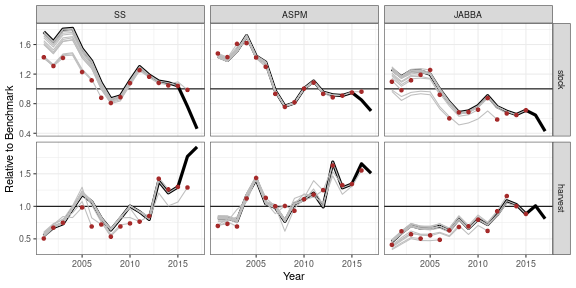
\includegraphics[width=6in]{figures/final-retro-1.png}}

\subcaptionbox{{b) 3-step ahead\newline}\label{fig:reto3}}{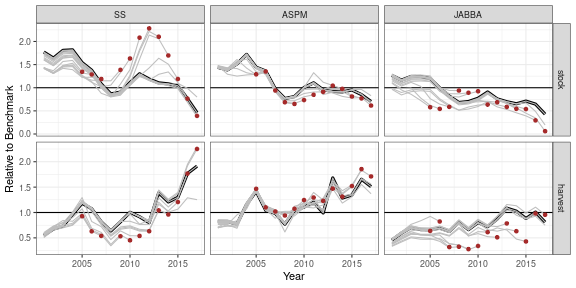
\includegraphics[width=6in]{figures/final-retro3-1.png}}

\caption{Hindcasts by a) 1 -step and b) 3-step ahead for Stock Synthesis (SS),  Age-Structure Equilibrium Model (ASPM), and Bayesian state-space biomass dynamics model (JABBA).  The thick solid line represent the model estimates for relative stock quantities $stock$ and $harvest$ relative to $MSY$ benchmarks ($SSB$ and instantaneous fishing mortality for SS and ASPM and total biomass and harvest rate for JABBA). The points indicate the terminal years of the peels.}\label{fig:retro}
\end{figure}

\begin{figure*}[htbp]
\centering
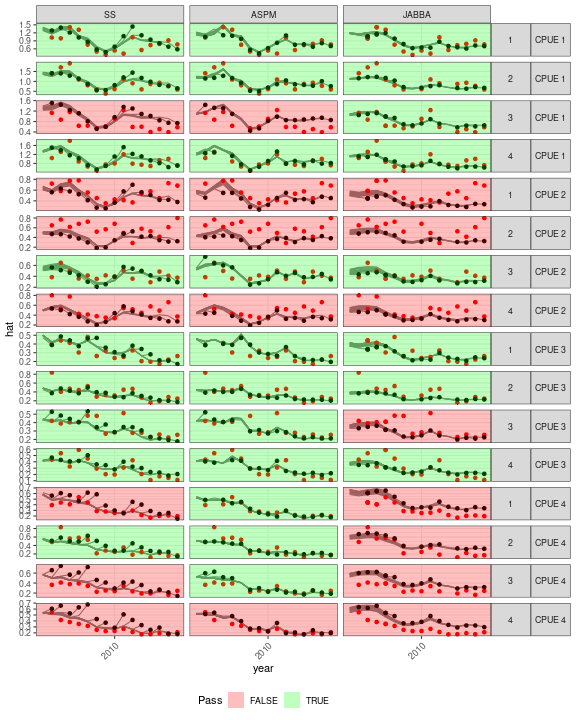
\includegraphics[width=6in]{figures/final-hy-plot-1.png}
\caption{Hindcasts with one year ahead projections for CPUE indices by region and quarter. Green backgrounds indicate that the CPUE index passes Mean Absolute Scaled Error (MASE < 1) criterion, or failed (red) otherwise. Red dots are the observed CPUE values and thin lines are the fits with terminal hincast year indicated by a solid point.}
\label{fig:hy}
\end{figure*}

\begin{figure*}[htbp]
\centering
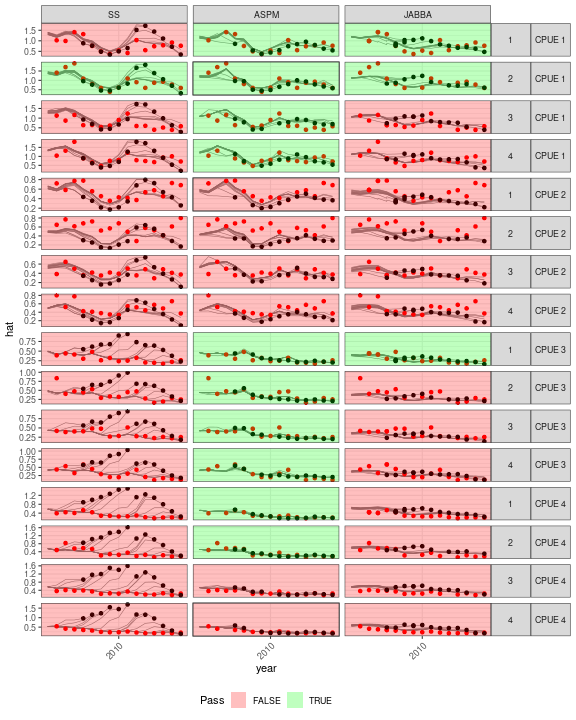
\includegraphics[width=6in]{figures/final-hy3-plot-1.png}
\caption{Hindcasts for 3 year ahead projections for CPUE indices by region and quarter. Green backgrounds indicate that the CPUE index passes Mean Absolute Scaled Error (MASE < 1) criterion, or failed (red) otherwise. Red dots are the observed CPUE values and thin lines are the fits with terminal hincast year indicated by a solid point.}
\label{fig:hy3}
\end{figure*}

\begin{figure*}[htbp]
\centering
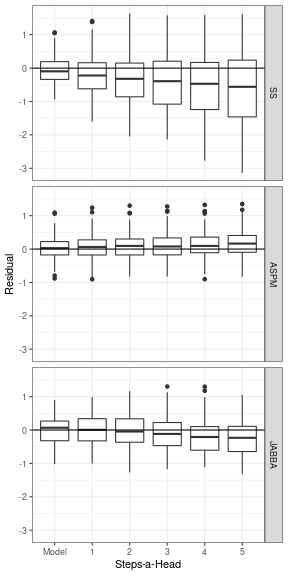
\includegraphics[width=4in]{figures/final-rsdl-1.png}
\caption{ Boxplots showing model residuals and prediction residuals for 1,2,3,4 and 5 year ahead projections, pooled for all CPUE indices across regions and quarters.}
\label{fig:residuals}
\end{figure*}

%\clearpage
%\newpage
%\subsection{Appendix}
%\label{metrics}

%\appendix* 
 %\subsection{Metrics}
%Indices of abundance are a key contributor to the overall likelihood when fitting stock assessment models to data. The Sum of Squared Errors (SSE) between observed and predicted indices in log-space is the measure of fitness. When comparing models, however, the SSE is problematic because complex models tend to have many parameters to allow flexibility when fitting, which may result in a low SSE due to overfitting. Therefore, information criteria, such as AIC, have been developed to aid in model selection. AIC is only a relative measure of the appropriateness of models, and additional diagnostic tests are required for model validation. This is of particular importance for stock assessment models where only a single historical data set exists, and the system can not be observed directly.

Therefore in stock assessment, a standard diagnostic is to evaluate retrospective bias as proposed by \cite{mohn1999retrospective}. As described in earlier sections, the retrospective analysis can be conducted by sequentially refitting the model to reduced data sets by removing some recent years' data to see if there are any systematic pattern within a model. The retrospective bias is then evaluated using the so-called Mohn's rho as 

\begin{equation}
\label{eqn:mohn0}
\rho_M = \disp \sum_{t=T-n}^{T-1} \frac{\hat{y}_{(1:t),t}-\hat{y}_{(1:T),t}}{\hat{y}_{(1:T),t}}, 
\end{equation}

where $\hat{y}$ denotes in general a value like estimated biomass, 1+population size, or predicted abundance index, and the value with suffix $\hat{y}_{(1:t^\prime),t}$ means such a value estimated at time $t$ of a full series from 1 to $T$ using a retrospective data window from 1 to $t^\prime (\leq T)$. In this paper, we will use a variant of the original $\rho$ as the mean (average) like 
\begin{equation}
\label{eqn:mohn}
\rho_{Mr} = \disp \frac{1}{n} \sum_{t=T-n}^{T-1} \frac{\hat{y}_{(1:t),t}-\hat{y}_{(1:T),t}}{\hat{y}_{(1:T),t}} 
\quad \mbox{[rho for retro-bias]}, 
\end{equation}
This metric is an average of relative differences at the final time of each window. Therefore it is a measure of relative retrospective `bias' (scale-free) in a statistical sense. The metric tends to be applied not on the log but the original scale because both the directions of positive and negative biases are regarded as being equivalent. 

To evaluate the absolute prediction error for the following can be used
\begin{equation}
\label{eqn:mohn3}
|\rho_p| = \disp \frac{1}{n-S+1} \sum_{t=T-n}^{T-S}
\frac{\left| \hat{y}_{(1:t),t+S}-\hat{y}_{(1:T),t+S} \right|}{\hat{y}_{(1:T),t+S}}. 
%\ \mbox{[rho for projection-absolute-error]}
\end{equation} 

Hindcasting, which is the primary focus in this paper is a form of retrospective cross-validation, and therefore an extension of retrospective analysis which projects several steps forward beyond the retrospective data window to quantify the prediction skill of a model. Theoretically, the projection period is to the end of the historical time period. However, in practice, the step size is one or several years ahead reflecting the requirements for robust management advice, and considering non-small process stochasticity in fishery population dynamics and non-ignorable extents of observation uncertainty. For evaluating prediction skill, we propose several metrics for model-dependent and model-free validations.

We  define `retro-period' and `hc-period' as `the period of shrunken data set for retrospective model fitting' and `future time period with a certain projection step (say $S \geq 1$) for hindcasting after retro-period''. And let $\hat{y}_{(1:t),t+S}$ be an projected value at time $t+S$ in an hc-period based on the conditioned model with data in a retro-period $(1,t)$. 

\vspace{0.2cm} \noindent
{\it Modified Mohn's rho for prediction bias and absolute error:}\\
\begin{equation}
\label{eqn:mohn2}
\rho_p = \disp \frac{1}{n-S+1} \sum_{t=T-n}^{T-S} 
\frac{\hat{y}_{(1:t),t+S}-\hat{y}_{(1:T),t+S}}{\hat{y}_{(1:T),t+S}} 
\ \mbox{[rho for projection-bias]}
\end{equation} 

This is a simple extension of Mohn's rho to evaluate the prediction skill of a model because all the values are produced under the model assumption. In this sense, it is a model-dependent consistency check of prediction skill. To evaluate the absolute prediction error for the following can be used
\begin{equation}
\label{eqn:mohn3}
|\rho_p| = \disp \frac{1}{(n-S+1)} \sum_{t=T-n}^{T-S}
\frac{\left| \hat{y}_{(1:t),t+S}-\hat{y}_{(1:T),t+S} \right|}{\hat{y}_{(1:T),t+S}}. 
\ \mbox{[rho for projection-absolute-error]}
\end{equation} 

There are problems with the use of relative error, since for reference model estimates which are low relative to the alternative model, i.e. $X_{ref} < X_{p}$, there is no upper limit, while for $X_{ref} > X_{p}$ the error cannot exceed 1.0. Therefore the chosen metric puts a heavier penalty on negative than on positive errors, i.e. historical underestimates. This means that when comparing models estimates, those that are low will be preferred. This problem can be overcome by using the logarithm of the ratio instead i.e. 
\begin{equation}
\label{eqn:re}
log\frac{X_{p}}{X_{ref}}
\end{equation}

which also leads to better statistical properties.


\vspace{0.2cm} 
The next three metrics are used for model-free validation, i.e. comparing predictions with observations. The error is defined as the difference between the predicted ($\hat{y}_{(1:t),t+S}$) and observed $y_{t+S}$) values, such as the model-based predicted CPUE using a retro-period data and observed CPUE used for model fitting. 

\vspace{0.2cm} \noindent
{\it Mean Absolute Percentage Error (MAPE) for projection:}
\begin{equation}
\label{eqn:mape}
MAPE = \disp \frac{1}{n-S+1} \sum_{t=T-n}^{T-S}
\frac{\left| \hat{y}_{(1:t),t+S}-y_{t+S} \right|}{y_{t+S}} \times 100 
\end{equation} 
A simple extension of the modified Mohn's rho for quantifying the relative difference between predictions and observations. This metric is also a scaled version of Mean Absolute Error (MAE). A problem with the MAE is that the relative size of the error is not always obvious. Sometimes it is hard to distinguish a big error from a small error. The MAPE can be calculated to allow forecasts of different series in different scales to be compared.

\vspace{0.2cm} \noindent
{\it Root Mean Squared Error (RMSE) for projection error:}\\
As an alternative measure of distance, the Mean Squared Error (MSE) is also commonly used in statistical literatures. To make comparison easier, the following squared root variant of MSE can be used: 
\begin{equation}
\label{eqn:rmse}
RMSE = \disp \sqrt{ \frac{1}{n-S+1} \sum_{t=T-n}^{T-S} 
\left( \hat{y}_{(1:t),t+S}-y_{t+S} \right)^2 }
\end{equation} 

In comparison to $\rho_p$ and MAPE, RMSE is not scale-invariant and can be influenced by large discrepancies in a single data point. A useful feature, however, that the squared RMSE can, in general, be expressed,  for a notational simplicity if we set $S$ at 1, as

\begin{equation}
\label{eqn:rmse2}
\begin{array}{lcl}
\vspace{0.1cm}
{RMSE}^2 &=& \disp \frac{1}{n} \sum_{t=T-n}^{T-1} \left( \hat{y}_{(1:t),t+1}-y_{t+1} \right)^2 \\
\vspace{0.1cm}
&=& \disp \frac{1}{n} \sum_{t=T-n}^{T-1} \left( \hat{y}_{(1:t),t+1}-y_{t+1} - \bar{E} \right)^2 + \bar{E}^2 \\
&=& \disp E^{\prime 2} + \bar{E}^2
\end{array}
\end{equation}
where 
\begin{equation}
\begin{array}{lcl}
\vspace{0.1cm}
\bar{E} &=& \disp \frac{1}{n} \sum_{t=T-n}^{T-1} \left( \hat{y}_{(1:t),t+1}-y_{t+1} \right), \\
\vspace{0.1cm}
E^{\prime 2} &=& \disp \frac{1}{n} \sum_{t=T-n}^{T-1} \left( \hat{y}_{(1:t),t+1}-y_{t+1} - \bar{E} \right)^2.
\end{array}
\end{equation}
The centred mean squared error, $E^{\prime 2}$ can be also expressed as 
\begin{equation}
E^{\prime 2} = \sigma_o^2 + \sigma_f^2 - 2\sigma_o \sigma_f Cor,
\end{equation}
where $\sigma_o$ and $\sigma_f$ are respectively the standard deviation of observation $y_t$ and prediction, and $Cor$ is the correlation between them. This means that $E^\prime$, $\rho$ and $\sigma_f$ can be summarised simultaneously \parencite{taylor2001summarizing}. Taylor diagrams provide a concise statistical summary of how well patterns match each other and are therefore useful for evaluating multiple aspects or in gauging the relative skill of different models \parencite{griggs2002climate}. It should be remarked that RMSE can be extended for a percentage measure as MAPE, but for the reason stated below, we use RMSE as defined above 

\vspace{0.2cm} \noindent
{\it Mean absolute scaled error (MASE) for projection:}\\ 
A more robust and easier to interpret statistic for evaluating prediction skill is the MASE \parencite{hyndman2006another}. MASE evaluates a model's prediction skill relative to a na\" {i}ve baseline prediction, based on previous observation. A prediction is said to have skill if it improves the model forecast compared to the baseline. A widely used baseline forecast for time series is the persistence algorithm that takes the value at the previous time step to predict the expected outcome at the next time step as a na\ "{i}ve in-sample prediction, i.e. tomorrow weather will be the same as today. The original definition of MASE for 1-step ahead prediction is 
\begin{equation}
\label{eqn:mase}
{MASE=\frac{\disp \frac{1}{n} \sum_{t=T-n}^{T-1} \left| \hat{y}_{(1:t),t+1}-y_{t+1} \right|}
{\disp \frac{1}{n-1} \sum_{t=T-n+1}^{T-1} \left|y_{t+1}-y_{t}\right|}}, 
\end{equation}
and this can be extended as \toshi{actually not very much straightforward but seems as below}
\begin{equation}
MASE=
\frac{\disp \frac{1}{n-S+1} \sum_{t=T-n}^{T-S}  \left| \hat{y}_{(1:t),t+S}-y_{t+S} \right|}
{\disp \frac{1}{n-S} \sum_{t=T-n+1}^{T-S} \left|y_{t+S}-y_{t}\right|}. 
\end{equation} 
The MASE has the desirable properties of scale invariance, predictable behaviour, symmetry, interpretability and asymptotic normality. Compared to MAPE, which relies on the division by observations for scaling, MASE does not necessarily skew its distribution even when the observed values are close to zero. MASE is also easier to interpret as a score of 0.5 indicates that the model forecasts are twice as accurate as a na\''{i}ve baseline prediction; the model thus has prediction skill.
\vspace{0.2cm} 
The best statistical measure to use depends on the objectives of the analysis and using more than one measure can be helpful in providing insight into the nature of observation and process error structures. Here for the evaluation of models, we will use the following metrics: 

\begin{itemize}
\item Original Mohn's rho ($\rho$) for checking the retrospective bias \\
\vspace{-0.3cm}
\item Modified Mohn's rho for prediction \toshi{bias and absolute error, which? both might be meaningful though but it becomes noisy...} as checking model-based self-consistency check \\
\vspace{-0.3cm}
\item MASE and RMSE for model-free validation with different angles. 
\end{itemize}


\end{document}

We wish to submit this paper for the special issue in commemoration of Sidney Holt, however, if not thought appropriate we would like it to be considered for a regular issue. 

The reason for submission to the special issue is because of discussions at the World Fisheries Conference (Cadrin and Dickey-Collas, 2014) where Sidney argued that the definition of stock assessment was ``The description of the characteristics of a 'stock' so that its biological reaction to being exploited can be rationally predicted and the predictions tested"  There was a lot of discussion but no resolution.

Our support for Sidney's reasoning was because this explicitly recognises that an aim of stock assessment is to provide the basis for the long-term sustainable management of fisheries, which Sidney's work laid the foundations for. Stock assessment, therefore, requires making and validating probabilistic estimates of stock status and forecasts of the consequences of management actions". This prompted a lot of debate but no clear conclusion, and we have written this paper in memory of Sidney.

Cadrin, Steven X and Mark Dickey-Collas (2014). “Stock assessment methods for sustainable fisheries”. In:ICES Journal of Marine Science72.1, pp. 1–6

